\usetikzlibrary{arrows}
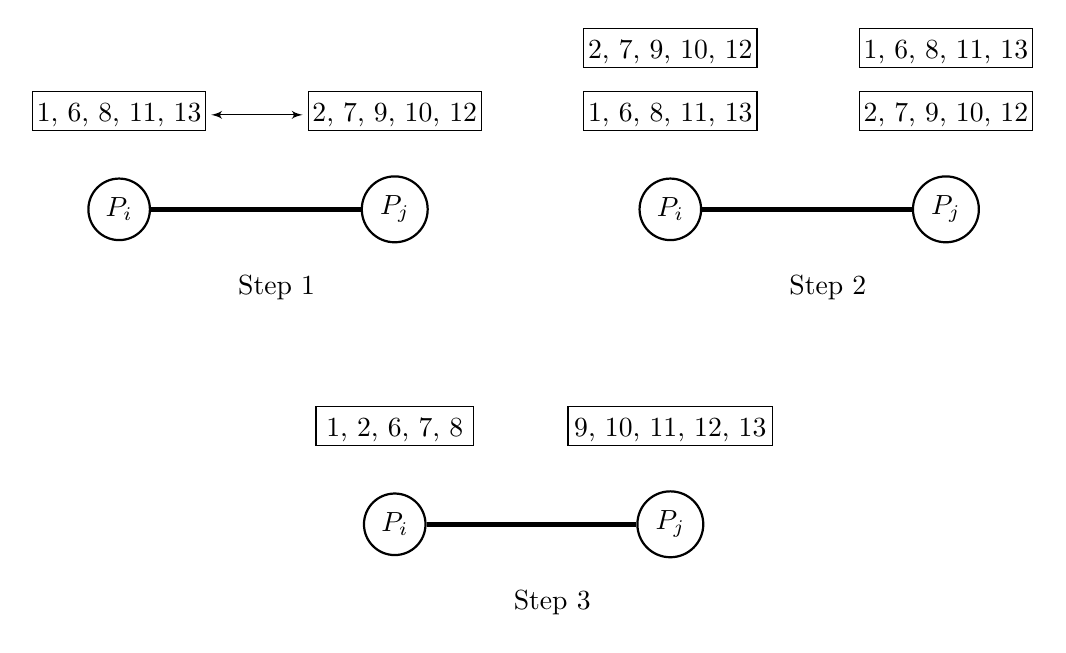
\begin{tikzpicture}

% \node (v1) at (-5,0) {$a_i$};
% \node (v2) at (-2,0) {$a_j$};

\draw (-6.6,0) rectangle +(2.2,0.5);  
\node (v1) at (-5.5,0.2) {1, 6, 8, 11, 13};
\draw (-3.1,0) rectangle +(2.2,0.5);  
\node (v2) at (-2,0.2) {2, 7, 9, 10, 12};

\node[draw, thick, circle] (P1) at (-5.5,-1) {$P_i$};
\node[draw, thick, circle] (P2) at (-2,-1) {$P_j$};

\draw [latex'-latex', double] (v1) edge (v2);

\draw[ultra thick]  (P1) edge (P2);

\node at (-3.5,-2) {Step 1};

\begin{scope}[shift={(7,0)}]

%\node (v1) at (-5,0) {$a_i,a_j$};
%\node (v2) at (-2,0) {$a_j,a_i$};

\draw (-6.6,0) rectangle +(2.2,0.5);  
\node (v1) at (-5.5,0.2) {1, 6, 8, 11, 13};
\draw (-3.1,0.8) rectangle +(2.2,0.5);  
\node (v12) at (-2,1) {1, 6, 8, 11, 13};

\draw (-6.6,0.8) rectangle +(2.2,0.5);  
\node (v21) at (-5.5,1) {2, 7, 9, 10, 12};
\draw (-3.1,0) rectangle +(2.2,0.5);  
\node (v2) at (-2,0.2) {2, 7, 9, 10, 12};

\node[draw, thick, circle] (P1) at (-5.5,-1) {$P_i$};
\node[draw, thick, circle] (P2) at (-2,-1) {$P_j$};

\draw[ultra thick]  (P1) edge (P2);

\node at (-3.5,-2) {Step 2};
\end{scope}

\begin{scope}[shift={(3.5,-4)}]

%\node (v1) at (-5,0) {$\min(a_i, a_j)$};
%\node (v2) at (-2,0) {$\max(a_i, a_j)$};

\draw (-6.5,0) rectangle +(2,0.5);  
\node (v1) at (-5.5,0.2) {1, 2, 6, 7, 8};
\draw (-3.3,0) rectangle +(2.6,0.5);  
\node (v2) at (-2,0.2) {9, 10, 11, 12, 13};

\node[draw, thick, circle] (P1) at (-5.5,-1) {$P_i$};
\node[draw, thick, circle] (P2) at (-2,-1) {$P_j$};

\draw[ultra thick]  (P1) edge (P2);

\node at (-3.5,-2) {Step 3};
\end{scope}

\node at (-6.5,0) {};
\end{tikzpicture}